\documentclass[aps,prb,twocolumn,superscriptaddress,floatfix,longbibliography,citeautoscript]{revtex4-2}

% Conveniently, the citeautoscript option in the revtex4-2 class toggles the spacing & punctuation automatically for superscript vs. bracketed citations. Place citations as if they were in [].
% Uncomment the line below to do superscript citations.
% \setcitestyle{super}

\usepackage{amsmath,amssymb} % math symbols
\usepackage{bm} % bold math font
\usepackage{graphicx} % for figures
\usepackage{comment} % allows block comments
\usepackage[normalem]{ulem} % allows strikeout text, e.g. \sout{text}

% \usepackage{minted} % allows colored code
% \usepackage{textcomp} % This package gives the text quote '

\usepackage{enumitem}
\setlist{noitemsep,leftmargin=*,topsep=0pt,parsep=0pt}

\usepackage{xcolor} % \textcolor{red}{text} will be red for notes
\definecolor{lightgray}{gray}{0.6}
\definecolor{medgray}{gray}{0.4}
\definecolor{mRed}{RGB}{230, 0, 50}
\colorlet{newtextColor}{mRed}

\usepackage{hyperref}
\hypersetup{
colorlinks=true,
urlcolor= blue,
citecolor=blue,
linkcolor= blue,
}

% Code to add paragraph numbers and titles
\newif\ifptitle
\newif\ifpnumber
\newcounter{para}
\newcommand\ptitle[1]{\par\refstepcounter{para}
{\ifpnumber{\noindent\textcolor{lightgray}{\textbf{\thepara}}\indent}\fi}
{\ifptitle{\textbf{[{#1}]}}\fi}}
%\ptitletrue  % comment this line to hide paragraph titles
%\pnumbertrue  % comment this line to hide paragraph numbers

% Code for reviewer text
%\newcommand{\revtext}[1]{\textcolor{reviewColor}{#1}}
\newcommand{\revtext}[1]{\textit{#1}}

% Code to track changes
\newif\iftrackchanges
\newcommand{\newtext}[1]
    {\textcolor{\iftrackchanges newtextColor\else black\fi}{#1}}
\newcommand{\deltext}[1]
    {\iftrackchanges{\textcolor{newtextColor}{\sout{#1}}}\fi}
%\trackchangestrue  % comment to hide tracked changes

% Instead of making TONS of colored newtext, let's just put a colored line next to big blocks of new text.
\usepackage{mdframed}
\newmdenv[
  linecolor={\iftrackchanges newtextColor\else white\fi},
  linewidth=2pt,
  topline=false,
  bottomline=false,
  rightline=false,
  skipabove=\topsep,
  skipbelow=\topsep,
  leftmargin=-12pt,
  innertopmargin=0pt,
  innerbottommargin=0pt
]{newtextblock}

% Uncomment this line if you prefer your vectors to appear as bold letters.
% By default they will appear with arrows over them.
% \renewcommand{\vec}[1]{\bm{#1}}

% Command to mark text in blue/red and define common units
\newcommand{\blue}{\textcolor{blue}}
\newcommand{\red}[1]{\textcolor{red}{#1}}
\newcommand{\df}{\dfrac}
\newcommand{\mic}{\mu\mathrm{m}}
\newcommand{\nm}{\mathrm{nm}}
\newcommand{\mm}{\mathrm{mm}}
\newcommand{\mrm}[1]{\mathrm{#1}}
\newcommand{\la}{\langle}
\newcommand{\ra}{\rangle}
\newcommand{\pd}[1]{\partial_{#1}}
% Command for labeled equations with custom alignment
\newcommand{\leqalign}[2]{
    \begin{equation}
        \begin{aligned}
            #2
        \end{aligned}
        \label{#1}
    \end{equation}
}

\ptitletrue
\pnumbertrue

% Replace minted with listings if you don't want to install Pygments
\usepackage{listings}
\usepackage{graphicx}
\usepackage{float}
\usepackage{siunitx}
% minimum font size for figures
\newcommand{\minfont}{6}
\usepackage{subcaption}
% Author affiliations
\newcommand{\heng}{School of Engineering \& Applied Sciences, Harvard University, Cambridge, Massachusetts 02138, USA}
\newcommand{\hphys}{Department of Physics, Harvard University, Cambridge, Massachusetts 02138, USA}

% Allows rewriting the same title in the supplement
\newcommand{\mytitle}{Optical Tweezers and Brownian Motion}

\begin{document}

\title{\mytitle}

\author{Adam Pearl}
\email[]{apearl@college.harvard.edu}
\affiliation{\hphys}
\author{Nicholas Lyu}
\email[]{nicholaslyu@college.harvard.edu}
\affiliation{\hphys}
% \affiliation{\heng}

\date{\today}

\begin{abstract}
We assembled an optical tweezer using an inverted 
microscope objective and a Hitachi HL6501MG 658nm laser diode. 
Using the tweezer, we demonstrate 3D trapping of $3\mic$ 
microspheres in aqueous solutions and measured the trap depth 
of the tweezer as a function of different laser powers. 
Additionally, using a digital image tracking package 
to determine the spheres' locations over time, 
we analyzed the Brownian motion of microspheres and experimentally 
determined the Boltzmann constant to be $1.762 \pm 0.423 \cdot 10^{-22} \si{\joule\per\kelvin}$ in comparison 
to the established value $1.381\cdot 10^{-23} \si{\joule\per\kelvin}$. 
\end{abstract}

\maketitle

%%%%%%%%%%%%%%%%%%%%%%%%%%%%%%%%%%%%%%%%%%%%%%%%%%%%%%%%%%%%%%%%%%%%%%%%
\section{\label{sec:intro}Introduction}
Optical tweezers use a tightly focused laser beam to trap microscopic systems 
by electromagnetic gradient forces~\cite{Ashkin1986,Smith1999AJP}. 
They provide a powerful tool for manipulating microscopic and many-body 
quantum systems~\cite{bluvstein2022quantum, beugnon2007two}. 
In this experiment, we build a basic optical tweezer and imaging system analogous 
to the design outlined in ~\cite{Smith1999AJP}. 
We demonstrate trapping dielectric microbeads in an aqueous solution, 
and measure the trap depth at different laser powers. 
By tracking the bead motion using the Python package \textit{Trackpy}, 
we analyze the Brownian motion of the microspheres to 
experimentally determine the Boltzmann constant using calculations 
outlined in~\cite{nakroshis2003measuring}. 

Optical tweezers operate by focusing a laser beam to create a steep electromagnetic intensity gradient that exerts forces on nearby dielectric particles. In the ray optics regime, light rays that are refracted and reflected by a particle impart momentum, generating a net force that draws the particle toward the region of highest intensity near the focus~\cite{Ashkin1986,Smith1999AJP,nieminen_optical_2014}. Alternatively, when the particle size is much smaller than the wavelength, the induced dipole moment interacts with the spatial gradient of the electric field, resulting in a restoring force that similarly confines the particle. In both cases, with proper focusing and sufficient laser power, these forces overcome thermal fluctuations to enable stable three-dimensional trapping.

One of the main objectives of our experiment is to determine the trap depth of our optical tweezer as a function of laser power. To achieve this, we monitor the escape of a dielectric microsphere from the trap while subjecting it to a controlled oscillatory motion using a Piezoelectric stage (refered to as Piezo). By gradually increasing the oscillation frequency, we identify the minimum period at which the particle escapes, and then convert this escape time into an escape velocity based on the known amplitude of oscillation. Using the relationship between the escape velocity and the force required to overcome viscous drag, we estimate the maximum restoring force of the trap. Finally, by combining this force with the effective trap width—derived from the beam's focal properties and the microscope objective's numerical aperture—we calculate the trap depth. Detailed theoretical calculations are provided in Sec~\ref{sec:trapDepth}, with the experimental results discussed in Sec~\ref{sec:trapDepthMeasurement}.

Another objective of our experiment is to estimate the Boltzmann constant from the observed Brownian motion of microspheres, following the procedure outlined in~\cite{nakroshis2003measuring}. To accomplish this, we use the \textit{Trackpy} python package to identify microspheres across video frames, enabling the reconstruction of their trajectories. From these trajectories, we calculate the mean-squared displacement as a function of time and perform a linear regression through the origin to determine the slope, which is directly proportional to the thermal energy of the system. In Sec.~\ref{sec:BoltzTheory}, we derive the formulas for both the point estimates and the error analysis, accounting for uncertainties arising from particle tracking, temperature measurements, and other systematic effects. Detailed procedures for data collection, statistical analysis, and the final estimates are provided in Sec.~\ref{sec:boltzmannCalc}, where our analysis yields an experimental Boltzmann constant of $1.762 \pm 0.423 \cdot 10^{-22}\,\si{\joule\per\kelvin}$. This significant deviation from the accepted value motivates a further discussion of potential systematic errors and avenues for improving the experimental setup.
\begin{figure}
    \centering
    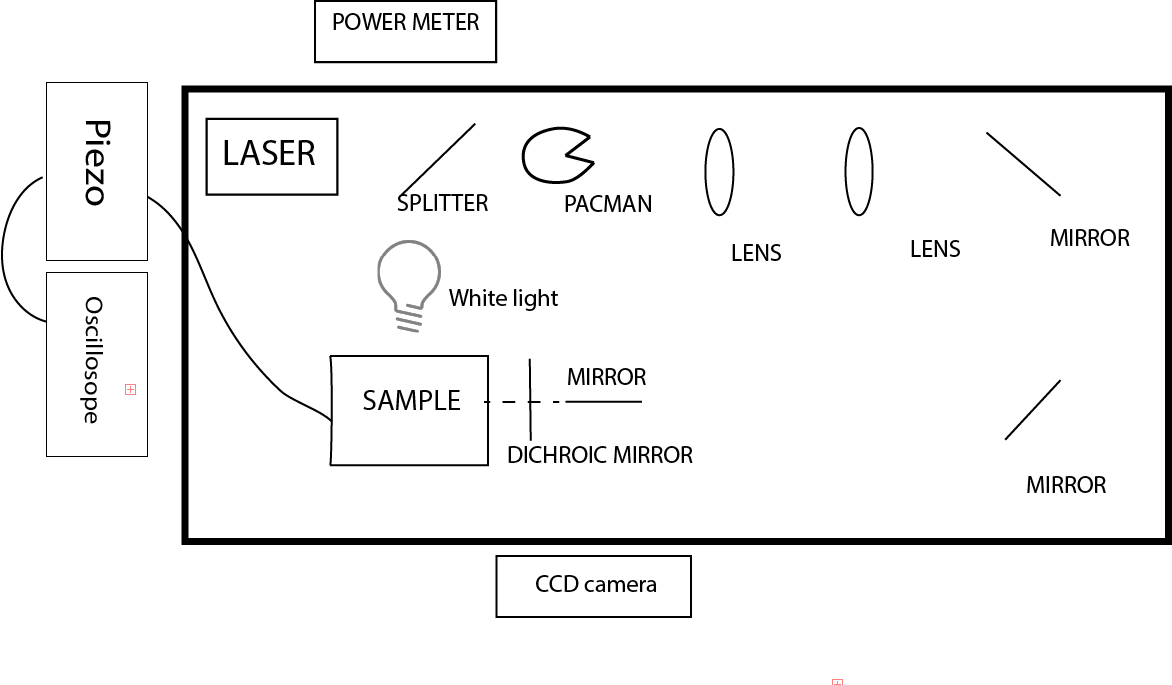
\includegraphics[width=1\linewidth]{./figs/tweezer-schmatic.png}
    \caption{Top down layout of the experiment.}
    \label{fig:circuit}
\end{figure}

\section{\label{sec:setup}Experimental Setup}
\subsection{\label{sec:imaging}Trapping and Imaging systems}
We followed the circuit in~\cite{OpticalTweezerInstructions} to shape 
the intial $658\nm$ beam from a Hitachi HL6501MG laser diode. 
The fiber-coupled initial laser is extracted and passed through a two-times 
magnification telescope lenses. 
The resulting beam is passed to an inverted microscope design to match the 
measured microscope objective diameter of $6\mm$. The optical table layout 
is depicted in Fig~\ref{fig:circuit}. 

\begin{figure}
    \centering
    \includegraphics[width=5cm]{./figs/imaging.png}
    \caption{Tweezer and imaging system. }
    \label{fig:tweezing}
\end{figure}
The tweezer system (Fig~\ref{fig:tweezing}) consists of a 
dichroic mirror which selectively reflects $658\nm$ light, an inverted, microscope objective which accepts collimated beams to produce $100\times$ magnification. 
The incoming trapping beam is reflected by the dichroic mirror and focused by the microscope objective onto the sample, which is placed on a 3-way translation stage with Piezo fine-control. A separate white-light illumination provided on 
the opposite direction of the sample passes through the dichroic mirror onto 
a Thorlabs camera, resulting in video imaging with a blue background. 
Compared to~\cite{OpticalTweezerInstructions} and~\cite{Smith1999AJP}, the objective of the microscope in our setup expects collimated beams; this allows us to omit 
a substantial portion of beam-shaping circuits. The camera imaging circuit involves a $50\mm$ focusing lens 
and camera directed at the microscope objective. Since both the imaging and laser beams are collimated, the focal plane of the camera roughly coincides with that for the trapping beam; this results in sharp imaging of the trapped particles. 

\begin{figure}
    \centering
    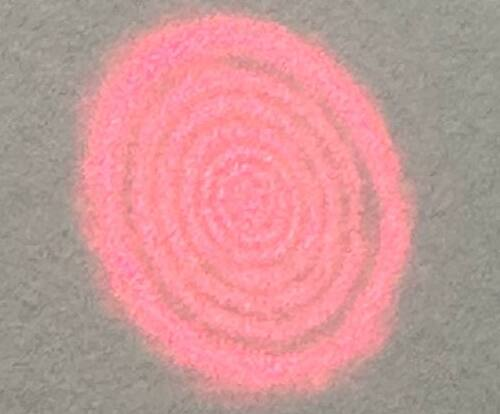
\includegraphics[width=5cm]{./figs/airy_pattern.jpg}
    \caption{Airy disc pattern of the trapping beam}
    \label{fig:airy}
\end{figure}
Upon visually inspecting the magnified trapping beam, we find it to be highly spherically symmetric but displaying an Airy disc pattern 
(Fig~\ref{fig:airy}) which deviate from the expected fundamental Gaussian mode. 
We haven't been able to visually identify this pattern from the fiber-coupled 
output prior to telescoping, which suggests that the diffraction pattern could be due to the use of small, half-inch lenses for magnification. 
It is also possible that the fiber-coupled output already contains higher-order modes prior to telescoping; the exact identification of the source of the diffraction pattern requires a beam camera. 

\subsection{Sample Preparation and Trap Calibration}
\begin{figure}[H]
    \centering
    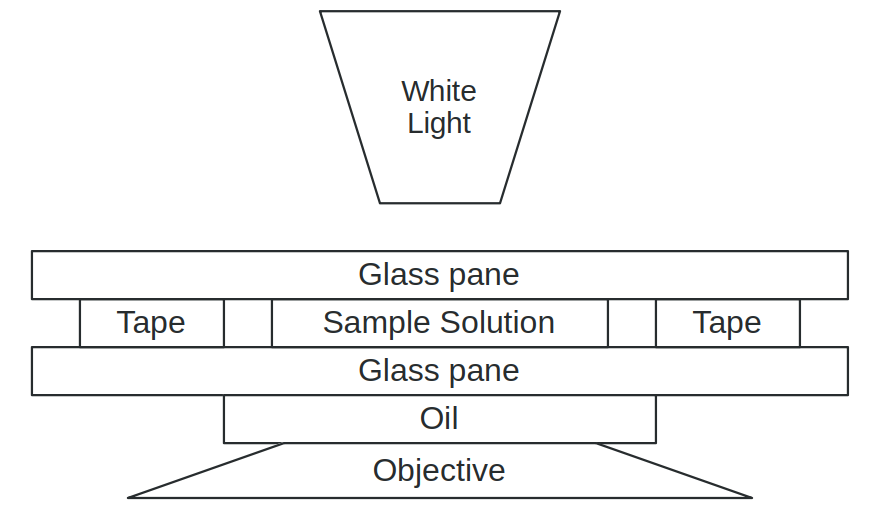
\includegraphics[width=1\linewidth]{./figs/sample_figure.png}
    \caption{Schematic of the trapped sample}
    \label{fig:sample}
\end{figure}
We use a sample of polystyrene microspheres diluted at a ratio of 5:1000 in de-ionized water. We use 3 micron beads as they are both large enough to easily be seen on camera as well as light enough to avoid sinking significantly. The solution is mixed and loaded between glass plates which are placed on the translation stage at the focus of the microscope (Fig~\ref{fig:sample}). 
\begin{figure}
    \centering
    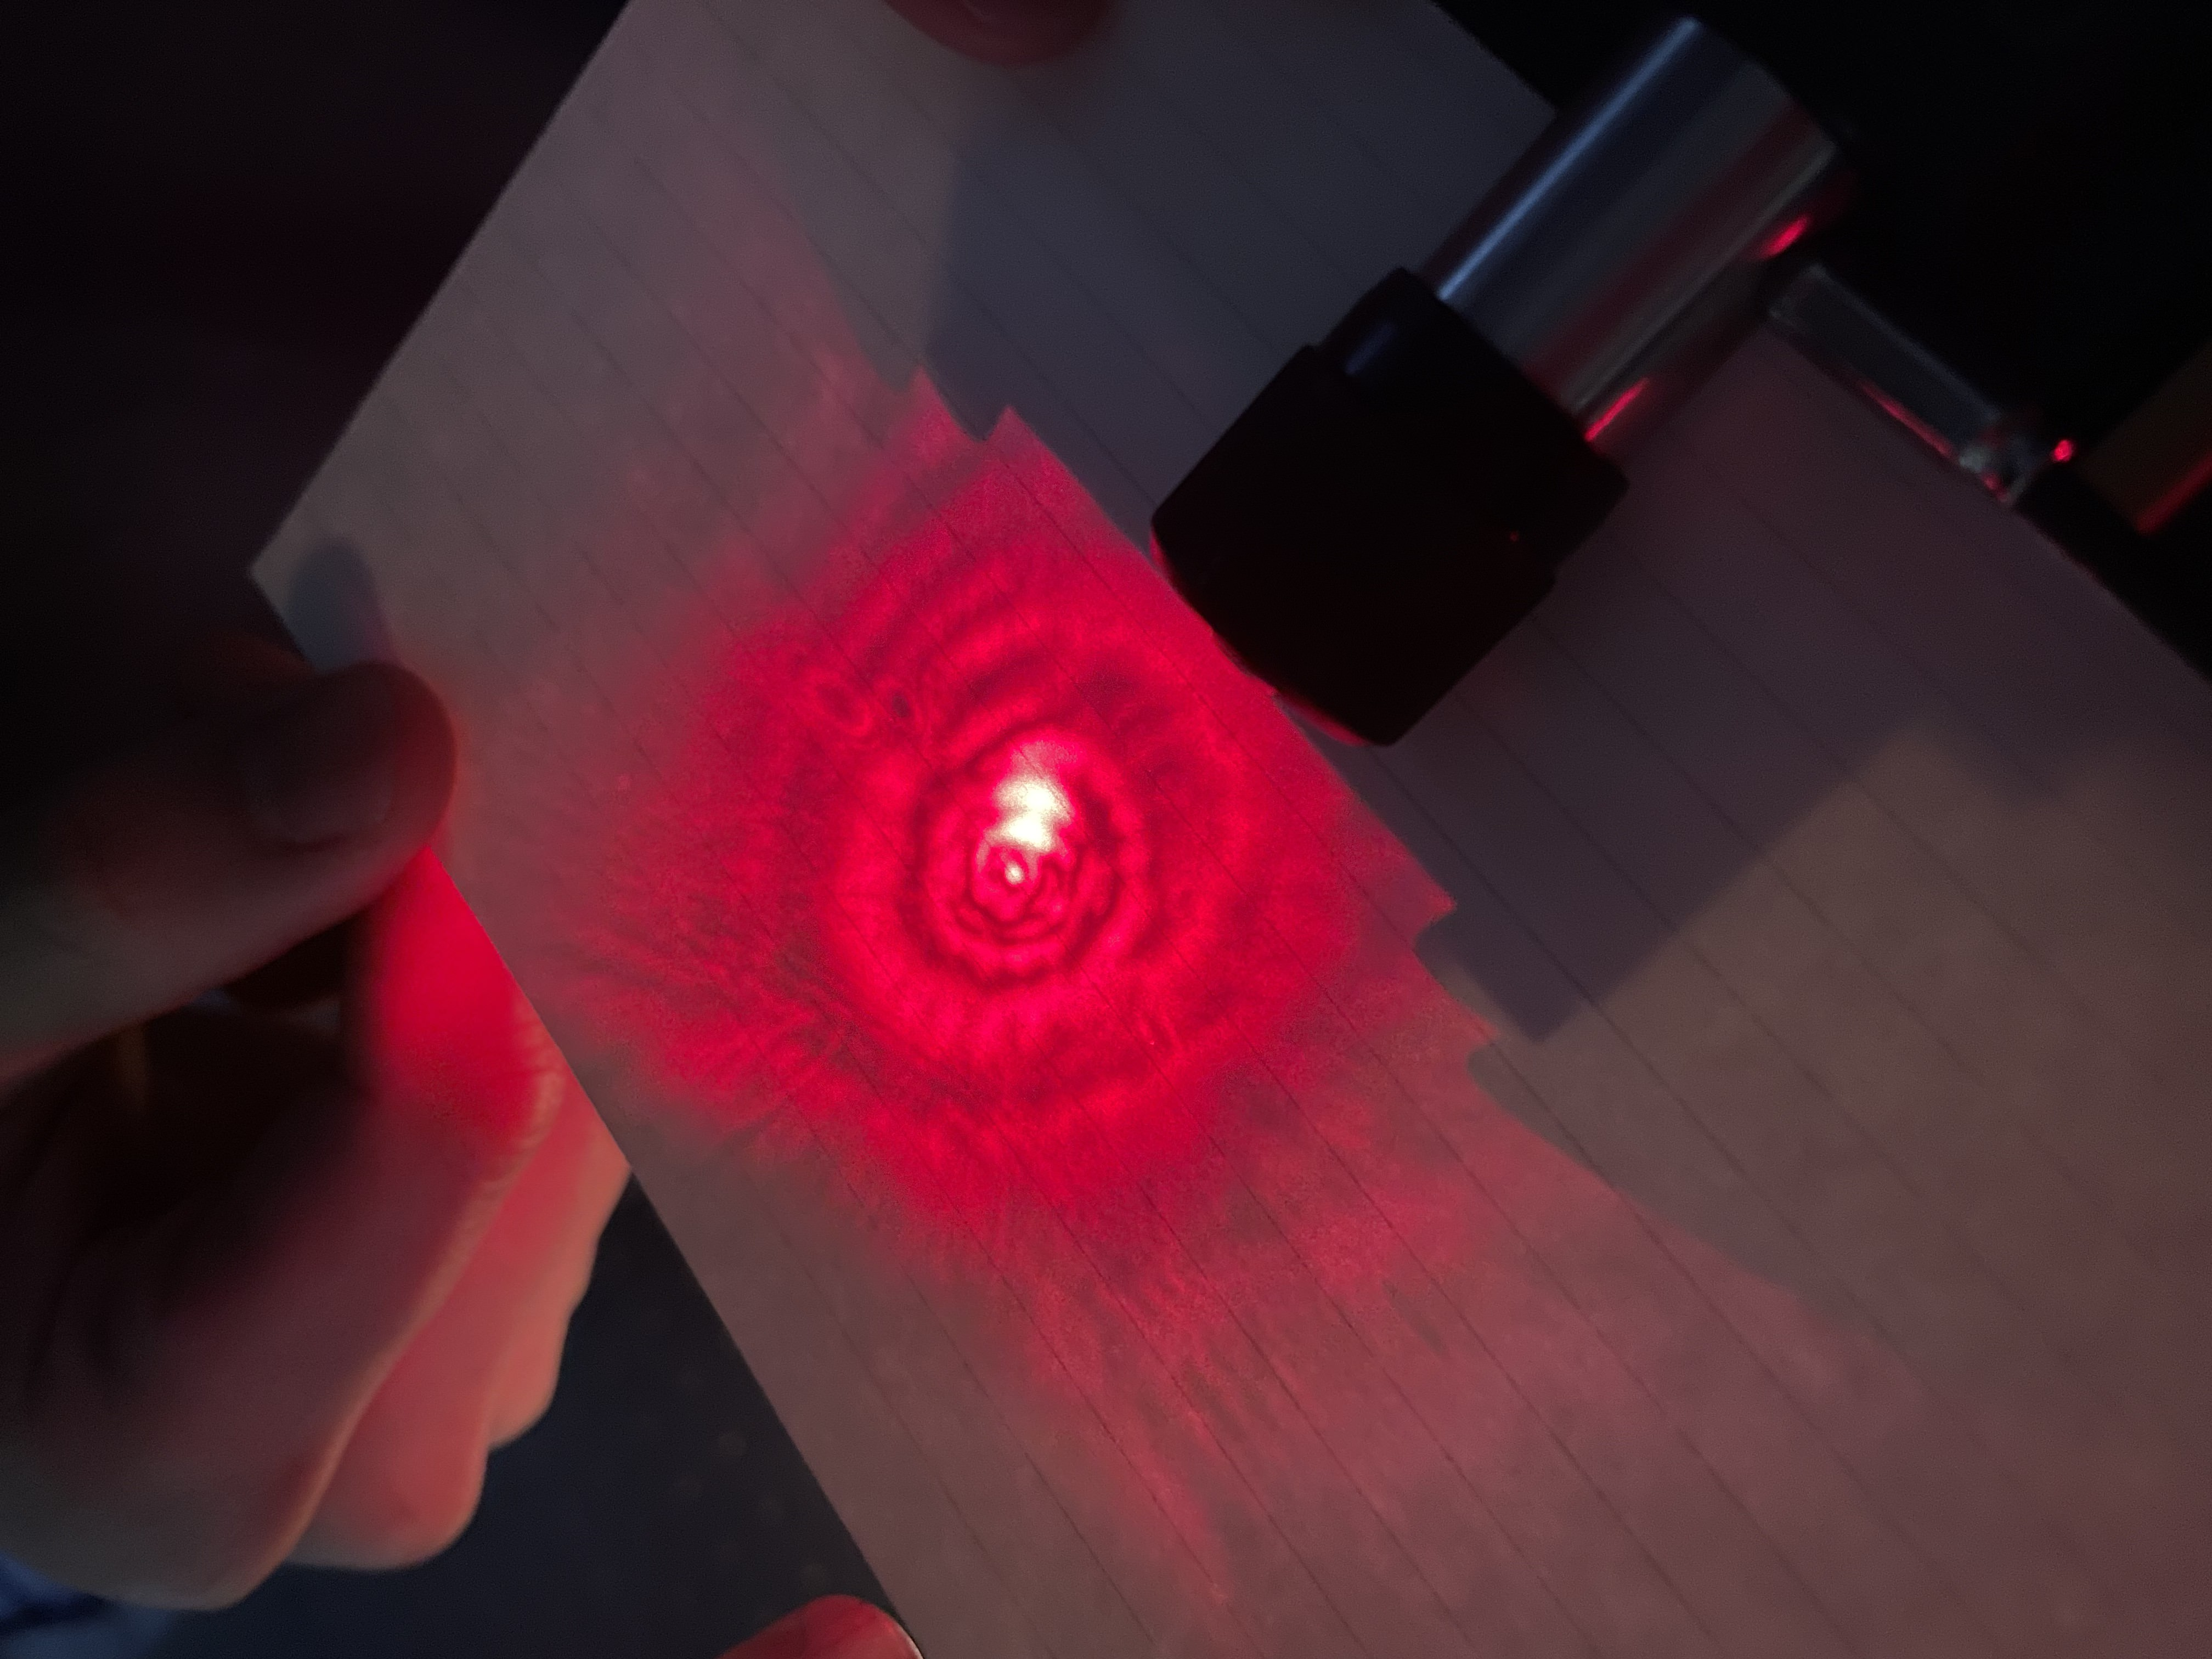
\includegraphics[width=5cm]{figs/diffraction.jpg}
    \caption{Diffraction pattern of a stably trapped microsphere. The imaging paper is placed above the sample and the microscope objective. The knob in the image adjusts the $x$-translation of the optical stage.}
    \label{fig:trapDiffractionPattern}
\end{figure}
The telescoping circuit is aligned with standard techniques; the beam is kept at a constant 
height and parallel to the breadboard axes. We align the vertical entry of the 
trap beam by adjusting the dicroic mirror to center the diffracted pattern on the sample site; 
this centers the $x$-$y$ dimension of our tweezer. 
The calibration of the $z$-axis proceeds in three steps: 
\begin{enumerate}
    \item To obtain the coarsest alignment, 
    we load a sample and inspect the trapping beam's diffraction 
    pattern through the sample. The microspheres appear as concentric circles with increasing diameter 
    as it nears the focus of the trapping beam. At a suitable coarse range of height, we observe large (in-focus) microsphere patterns suddenly attracted into the center then decrease in size as they escape along the $z$-axis. 
    \item We next fine-adjust the $z$-translation to ensure that the microspheres are subject to stable 3D trapping. 
    This is done by adjusting the $z$-axis until the trapped diffraction pattern remain stable (Fig~\ref{fig:trapDiffractionPattern}). 
    \item To fine-tune the trap, we image the trap (Figure~\ref{fig:trapCamera}) and turn on the PZT to induce circular motion of the samples. 
    For each $z$-displacement, we identify the maximum frequency at which the microsphere remains trapped and 
    optimizes this frequency. 
\end{enumerate}
\begin{figure} % The [H] forces the image to appear here
    \centering
    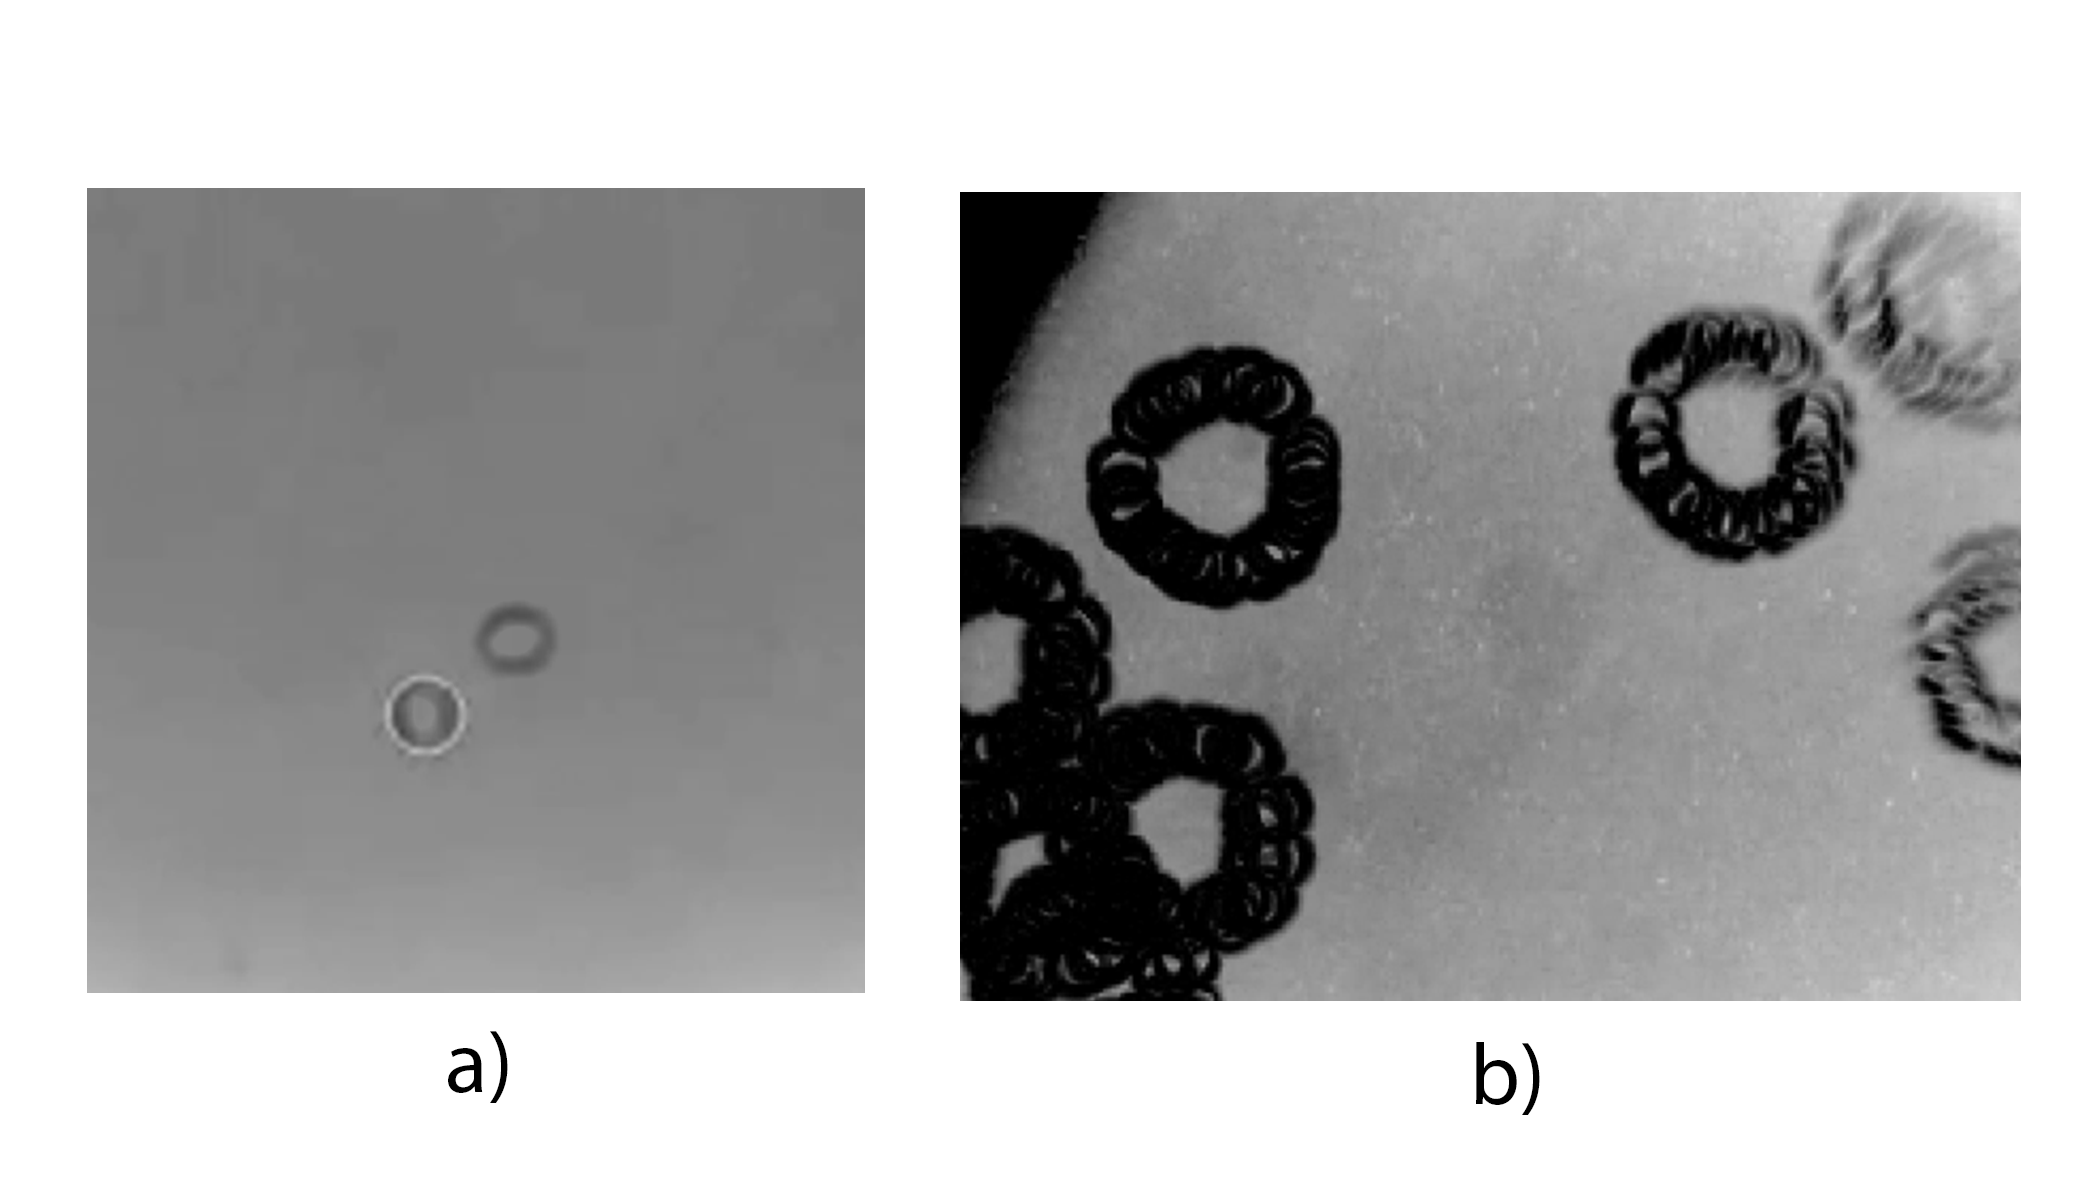
\includegraphics[width=1\linewidth]{./figs/bw.png}
    \caption{CCD captures. a) Overlayed images of a single particle before and after trap activation. Trap location is marked with a circle. b) Overlayed sequence of beads rotating due to a Piezo-induced driving force.}
    \label{fig:trapCamera}
\end{figure}
We also note that microspheres tend to sink to the bottom of the sample after several minutes. This implies that trapping is most easily identified during the first few minutes of loading a new sample, during which the greater $z$-uniformity of the microsphere distribution facilitates the identification of the focal plane. 

\subsection{Measuring Trap Depth \label{sec:trapDepth}}
The main objective of this experiment is to measure the trap depth - the kinetic energy a particle needs to escape a trap - as a function of laser power. In our optical tweezer experiment, we measure the Piezo driving frequency at which a particle caught in a trap escapes the trap as a function of laser power. In order to extract from these measurements a relationship between laser power and trap depth, we need to make some conversions. 
The path a particle follows is determined by the Piezo sine and cosine diving frequency. 

$$\boldsymbol{x}(t) = \left(A\cos(2\pi t /\tau), A\sin(2\pi t/\tau)\right)$$
And has a linear velocity of $v = \frac{2\pi A}{\tau}$, so the velocity at which a particle escapes from the trap is $v_{\text{esc}} = \frac{2\pi A}{\tau_{\text{esc}}}$.

The trap depth represents the binding energy of the trap, $D = F_{\text{max}}w_{\text{trap}}$. The maximum restoring force on the bead from the trap is inferred from the escape velocity; the trap width is jointly determined by the characteristics of the focused laser beam and the spheres.

In order for the trap to retain a bead it must provide a restoring force greater than or equal to the stokes drag caused by the solution moving relative to the bead given by $F_{S} = 6 \pi \eta r v$ where $\eta$ is the viscosity of the solution, which we approximate using $\eta\approx \SI{1e-3}{\newton\second\per\meter^2}$ using that of water at lab temperature (section~\ref{sec:boltzmannCalc}). 
Therefore $F_{\text{max}} = 6 \pi \eta r v_{\text{esc}}$. 
From \cite{Smith1999AJP}, an ideal lens with numerical aperture $NA$, passing through a medium with index of refraction $n$, focusing a collimated laser with wavelength $\lambda$ will produce a trap of width
$$w_{\text{trap}} \geq \frac{1.22 \lambda}{n} \sqrt{\left( \frac{n}{\text{NA}} \right)^2 - 1}$$. The trap restoring force is inversely proportional to $w_{\text{trap}}$, so for the same binding energy a trap with a larger width will be less strongly confining. $w_{\text{trap}}$ is minimized when the diameter of the indecent laser light at the objective is close to the diameter of the objective,$d_\text{objective} \approx D_\text{objective}$, such that the maximum amount of light is transferred \cite{Smith1999AJP}. After calibrating $d_\text{objective}$, we take the trap width to be the minimal trap width. Our inequality becomes an equality and the trap depth is given by

$$D = \frac{7.32 \pi \eta r v_{\text{esc}} \lambda}{n} \sqrt{\left( \frac{n}{\mrm{NA}} \right)^2 - 1}$$

where the factor of $7.32$ comes from multiplying dimensionless factors in the equations for $w_{\text{trap}}$ and $F_s$.
Our parameters are $\lambda = \SI{658}{nm}$, $\mrm{NA} = 1.25$, and the index of refraction of polystyrene is $n = 1.59$. 

The multiplicative error is 

$$ \sigma_D^2 = D^2 \left( \frac{\sigma_\eta^2}{\eta^2} + \frac{\sigma_A^2}{A^2} + \frac{\sigma_{v_{\max}}^2}{v_{\max}^2} \right) $$


\section{Boltzmann Constant Measurement}
\subsection{Particle tracking}
The CCD camera provides real-time videos of microspheres in the focal plane. 
The camera input is monitored using the ThorCams software; since ThorCams does not offer native 
video capture, we use a third-party screen-capture software to save the videos. 
We use the TrackPy~\cite{trackpy} python package to locate the spheres of interest and track their location over time. In order to determine the length scales in our videos, we compare the known $a=\SI{3}{\micro\meter}$ radius of the microspheres to their radius in pixels. There is an uncertainty on this conversion primarily due to the thick shell on the images of the spheres as seen in figure~\ref{fig:trapCamera} a). The ratio of the width of the shell to the diameter of the sphere gives an uncertainty of approximately $\sigma_a = \SI{0.72}{\micro\meter}$. 
% While this uncertainty is factored into the uncertainty on $A$ for the trap depth experiment, it is not factored into the uncertainty calculation for the Boltzmann constant (see \ref{sec:conclusion} ).

\subsection{Boltzmann Constant Estimation \label{sec:BoltzTheory}}
Assuming Brownian motion data $(x_j(t), y_j(t))_{j=1, \dots N}$ of $N$ particles for $t=t_1, \dots, t_m$, 
where $x_t, y_t$ are the displacement of the particles from their original position, 
we can estimate the mean-squared displacement of the particles as a function of time. 
\begin{equation}
    \langle R\rangle_t = \dfrac 1 N \sum_{j=1}^N x_j(t)^2 + y_j(t)^2 
\end{equation}
The measured two-dimensional mean-squared displacement is proportional to the drift time and Boltzmann constant via \citep[see][Eq. 3]{nakroshis2003measuring} 
\begin{equation}
    \la R^2(t)\ra = \dfrac{4k_B T}{6\pi \eta a}t \iff \hat k_B = \dfrac{6\pi \eta a}{4T} \cdot \widehat{\dfrac{\la R^2(t)\ra}{t}} 
    \label{eq:bolzCalc}
\end{equation}
here $k_B$ is the Boltzmann constant, $T$ is the temperature, $\eta$ is the viscosity of the solution, and 
$a$ is the spherical particle's radius. The ensemble-average formula is derived by solving for the equilibrium
mean squared displacement as a function of a dissipative drag force, which can be determined using Stokes' law
and the viscosity. Error sources include the temperature $\sigma_T$, viscosity $\sigma_\eta$, diameter $\sigma_a$, 
as well as the linear fit error $\sigma_\beta$. 

From equation~\ref{eq:bolzCalc}, we expect the observed expected mean-squared displacement $\la R^2(t)\ra$ 
to be a linear function of $t$. We estimate the slope $\beta = \la R^2(t)\ra / t$ using 
a univariate linear regression through the origin~\cite{BlitzsteinShephard2024}: 
given $(t_j, \la R^2(t_j))_{j=1}^N$, the point estimate is 
\leqalign{eq:boltzmannBeta}{
    \hat \beta = \dfrac{\sum_{j=1}^N t_j \la R^2(t_j)\ra}{\sum_{j=1}^N t_j^2}
}
The unbiased estimate of the residual standard deviation and the slope's error are, 
correspondingly, 
\leqalign{eq:boltzBetaError}{
    \hat \sigma^2 
    &= \dfrac 1 {n-1} \sum_{j=1}^N 
    \left[\la R^2(t_j)\ra - \hat \beta t_j \right]^2, \quad 
    \hat \sigma_{\beta} = \dfrac{\hat \sigma}{\sqrt{\sum_{j=1}^N t_j^2}}
}
However, we note that the formula above assumes homoskedasticity, i.e. 
the variance of $\la R^2(t)\ra$ is constant with respect to $t$. 
In practice, we observe that the variance of $\la R^2(t)\ra$ increases with 
$t$ (Figure~\ref{fig:dispCorrected}), violating the homoskedasticity assumption. 
To account for this, we use the heteroskedasticity-consistent estimate of 
$\beta$'s standard error, given by 
\leqalign{eq:boltzBetaErrorHet}{
    \hat \sigma_{\beta} = \dfrac{
        \sqrt{\sum_{j=1}^N t_j^2 \left[\la R^2(t_j)\ra - \hat \beta t_j\right]^2}
        }{\sum_{j=1}^N t_j^2}
}
Further recall that given $k_B = f(\eta(T), T, a, \beta)$ as in equation~\ref{eq:bolzCalc}, 
the error formula is 
\leqalign{eq:boltzErrorAbstract}{
    \hat \sigma_{k_B}^2 
    &= 
    \left(\sigma_T \dfrac{df}{dT}\right)^2 + 
    \left(\sigma_a \pd a f\right)^2 + 
    \left(\sigma_\beta \pd \beta f\right)^2 \\ 
    &= \dfrac{9\pi^2}{4T^2} \left[
        \beta^2 \sigma_a^2 \eta^2 + a^2 \sigma_\beta^2 \eta^2 + 
        \sigma_T^2 a^2\beta^2 \left(
            \eta'(T) - \dfrac{\eta}{T}
        \right)^2 
    \right] 
}
We use these formulas to estimate the Boltzmann constant experimentally in Sec~\ref{sec:boltzmannCalc}. 
\section{\label{sec:analysis}Experimental Results}
Our experimental data consists of the following: 
\begin{itemize}
  \item \textit{Trap depth analysis}: For laser driven at $I_{\mrm{LD}}$ in $\{80, 85, 90, 95, 100\} \, \mrm{mA}$, the minimum oscillation period at which microspheres remain stably trapped by the tweezer. We also use a power meter to record the laser power at each of these driving levels. 
  \item \textit{Boltzmann constant estimation}: 26 videos of $15\mrm s$ particle drifts, for $3\mic$ spheres in $5:1000$ sample of de-ionized water. We also record the temperature of the operational microscope apparatus, as a proxy for the sample temperature. 
\end{itemize}

\subsection{Trap depth measurement \label{sec:trapDepthMeasurement}}
\begin{figure}
    \centering
    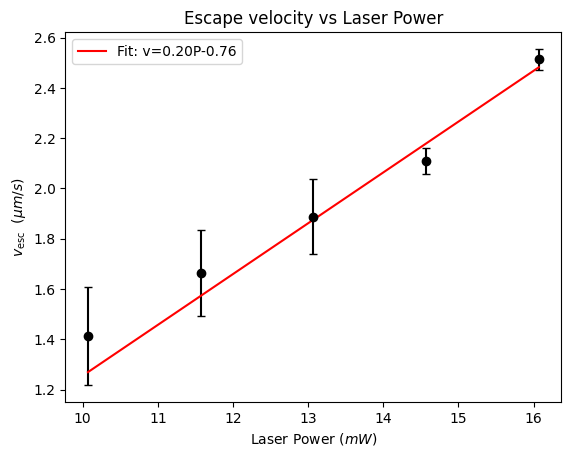
\includegraphics[width=0.3\textwidth]{figs/vesc.png}
    \caption{Escape velocity vs laser power. Linear fit $v = mP + b$ parameters : $m = 0.2\pm \SI{0.023}{\milli\meter\per\second\per\watt}$, $b = -0.76 \pm \SI{0.346}{\micro\meter\per\second}$. }
    \label{fig:plot1}

    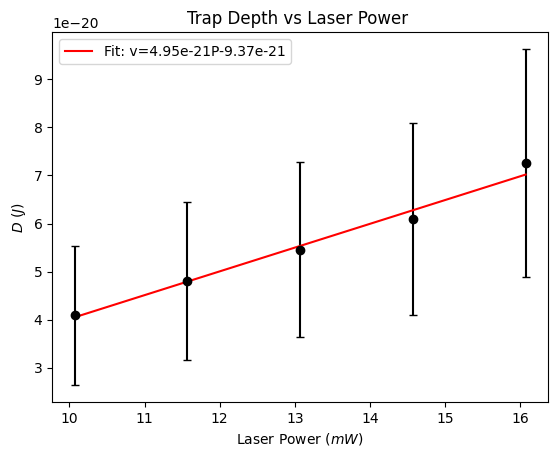
\includegraphics[width=0.3\textwidth]{figs/depth.png}
    \caption{Trap depth vs laser power (data pending). Linear fit $D = mP + b$ parameters : $m = (5.73 \pm 4.52 )\cdot 10^{-21} \si{\kilo\joule\per\watt}$, $b = (-1.085\pm 5.6734)\cdot 10^{-20} \si{\joule}$. }
    \label{fig:plot2}
\end{figure}
In order to measure $\tau_{\text{esc}}$, we first trap a microsphere with the Piezo turned off. We then initiate the Piezo and calibrate the trap such that it can hold the sphere at the minimum possible driving period. At each recorded value of power, we measure the minimum driving period at which the particle remains in the trap. Upon doing initial trials, we realized that the trap-depth versus driving current curves were offset from trial to trial. This is likely because our trap was sensitive to distance and fell out of calibration over time. We subsequently corrected this by recalibrating the trap at the beginning of every round of data collection sampling the range of $I_{\mrm{LD}}$. Only the calibrated data are used for analysis below. 

In order to measure $A$, we record videos of particles undergoing rotations and use image-analysis software to overlay particle paths over time (figure ~\ref{fig:trapCamera} b)). We measure the diameter in pixels and use the ratio of the diameter of the spheres in pixels to the diameter of the spheres in microns to convert to microns. This is repeated for multiple trails, and the measurement uncertainty is taken to be radius of the spheres, which was a larger uncertainty than the standard error on the measurement, $A = 4.6\mic \pm 1.5 \mic$. From section~\ref{sec:boltzmannCalc}, we estimate our uncertainty on $\eta$ to be $\Delta\eta =  \pm 2.2 \cdot 10^{-6}$ . However given our approximation of $\eta \approx 10^{-3}$ this uncertainty is much smaller than our precision on $\eta$ and so we set $\sigma^2_\eta = 0$.

In figures ~\ref{fig:plot1} and ~\ref{fig:plot2}, we observe linear trends between laser power and escape velocity, trap depth. The linear fit between laser power and trap depth is captured entirely by our error bars.



\subsection{Boltzmann constant estimate \label{sec:boltzmannCalc}}



\begin{figure}
    \centering
    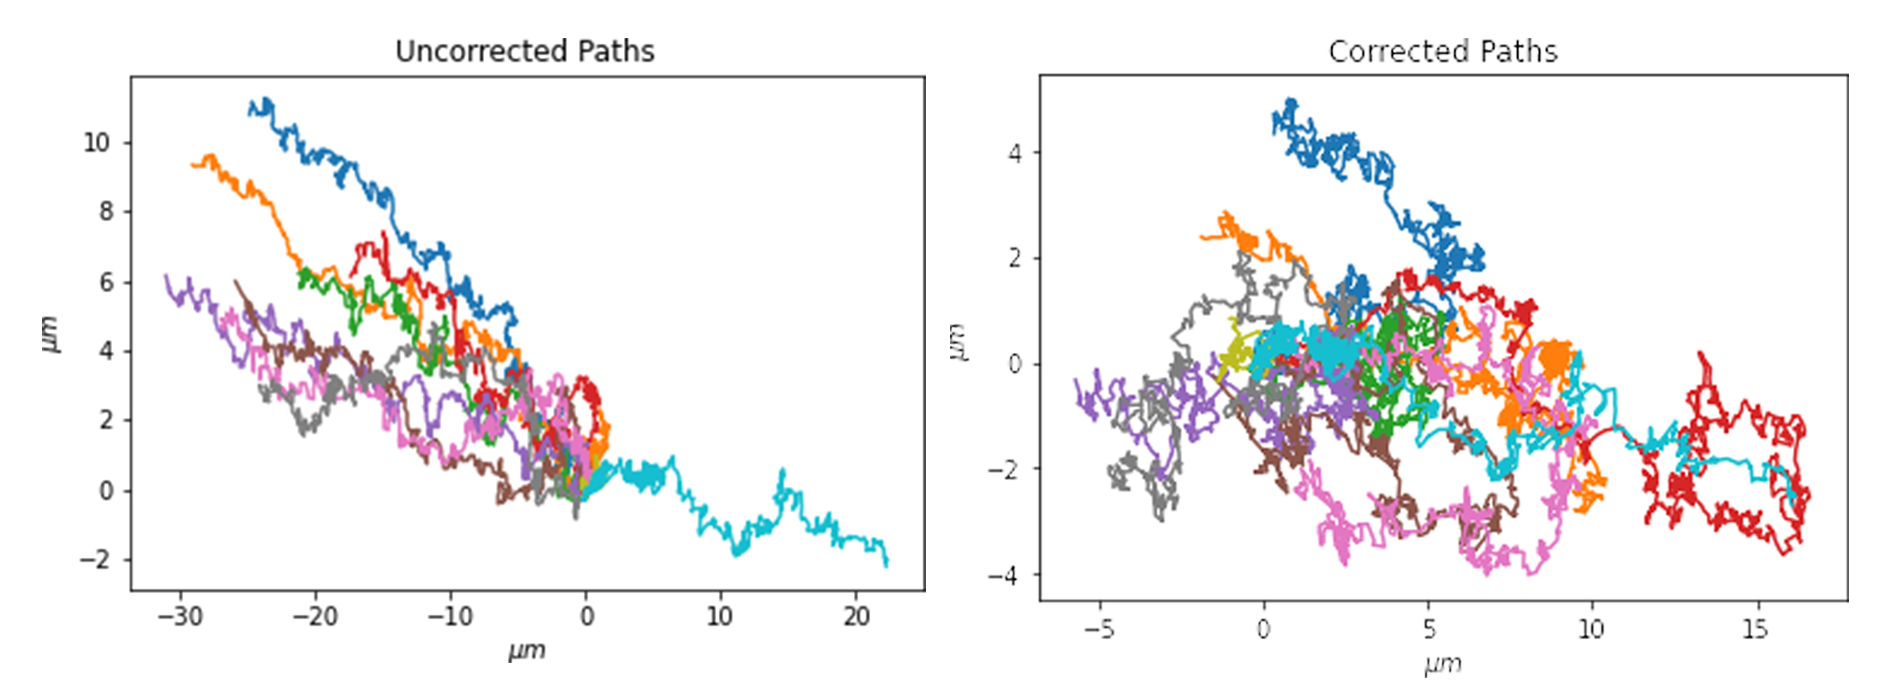
\includegraphics[width=1\linewidth]{./figs/paths.png}
    \caption{(Left) raw trajectory of $10$ tracked microspheres over $15$ seconds; the trajectories display significant drift. (Right) drift-corrected trajectories.}
    \label{fig:trajCorrected}
\end{figure}
We first filtered the original 26 recordings based on how long the particles can be reliably tracked by our tracking algorithm. Since the microspheres also undergo Brownian motion in the focal axis, beads are also prone to falling out of focus before drifting far in the $xy$ plane. We have been able to consistently track the displacements of $10$ particles in the videos. We imposed a uniform tracking time cutoff of 15 seconds which tracks the microspheres in all of the videos because a longer cutoff will introduce selection bias into the $z$-component of the Brownian motion. This leaves us with $10$ videos in which microspheres are all reliably tracked for $15$ seconds. 

Our first results showed a significant drift (Fig~\ref{fig:trajCorrected}). We collected two batches of data ($10$ and $16$ videos, respectively) over two days, each with a different physical microsphere sample. The different microsphere samples have different drifts, as evidenced by the distinct northwest vs. south-east drifts in the figure. The constant drift inflates the Boltzmann constant estimate by increasing the mean-squared displacement, and we correct for the drift by estimating the constant drift vector 
\[ 
    \hat{\mathbf v} = \df 1 {mT} \sum_{j=1}^m \mathbf{x}(T)_j, \quad T=\SI{15}{\second} 
\]
separately within each batch. The corrected trajectory are shown in Fig~\ref{fig:trajCorrected} (right). Based on the drift-corrected paths, we estimated the mean squared displacement as a function of time. The corrected displacements of each microsphere with respect to time are plotted in~\ref{fig:dispCorrected}. Note that the uncertainty in mean displacement increases with time, justifying the heteroskedastic slope error formula~\ref{eq:boltzBetaErrorHet}. 
\begin{figure}
    \centering
    \includegraphics[width=1\linewidth]{./figs/displacements.png}
    \caption{(Left) displacement from the trap origin as a function of time for each microsphere.  (Right) linear fit of the average squared displacement with respect to time. }
    \label{fig:dispCorrected}
\end{figure}
We estimate the sample temperature by observing the microscope temperature 
$T=20.3\pm 0.1\si{\degreeCelsius}$. To obtain the sample viscosity and its derivatives, we approximate the sample as water and 
used a reviewed \href{https://www.omnicalculator.com/physics/water-viscosity}{online viscosity calculator}
to obtain the viscosity point-estimates of water around $20.3\si{\degreeCelsius}$. 
\[ 
    \eta
    \begin{pmatrix}
        20.2 \\ 20.3 \\ 20.4 
    \end{pmatrix} \si{\degreeCelsius} 
    = 
    \begin{pmatrix}
        0.9968 \\ 0.9944 \\ 0.992
    \end{pmatrix} \si{ \milli \pascal \cdot \second}
\] 
Using these estimates, we estimate the viscosity derivative using central difference: 
\leqalign{eq:waterViscosity}{
    \eta'(\SI{20.3}{\degreeCelsius}) 
    &\approx \dfrac{\eta(\SI{20.4}{\degreeCelsius}) - \eta(\SI{20.2}{\degreeCelsius})}{\SI{0.2}{\degreeCelsius}}\\ 
    &\approx \SI{-0.024}{\milli \pascal \cdot \second\per\degreeCelsius}
}
The estimates of the remaining values in equation~\ref{eq:boltzErrorAbstract} are 
\leqalign{eq:boltzValues}{
    \hat \beta = 3.678 \pm \SI{0.012}{\micro\meter^2\per\second} \quad 
    a = 3\pm \SI{0.72}{\micro\meter}
}
The final estimates are (\href{https://www.wolframcloud.com/obj/nicholaslyu/Published/Notebok%20Calculations.nb}{Mathematica calculation)}: 
\leqalign{eq:boltzFinalEstimates}{
    \hat k_B &= 1.762 \cdot 10^{-22} \si{\joule\per\kelvin}, \,\,
    \sigma_{k_B} = 4.229 \cdot 10^{-23} \si{\joule\per\kelvin}
}
Comparing to the known Boltzmann value $k_B=1.3806\cdot 10^{-23}\mrm{J/K}$, we observe that we overestimated by an order of magnitude ratio of $\sim 11.8$. 


\section{\label{sec:conclusion}Discussion}


Our results yielded a predicted Boltzmann constant an order of magnitude larger than its true value. Despite this significant discrepancy, our uncertainties are an order of magnitude smaller than our predicted value, suggesting that systematic errors were the dominant source of error in our experiment.

One likely source of systematic error was particle drift, which we were unable to fully eliminate. This drift may have resulted from an improperly leveled table supporting our experimental setup, causing particles to move under the influence of gravity. Additionally, the construction of the sample pane introduced unavoidable inhomogeneities, and air gaps in the tape securing the panes may have contributed to a net fluid flow. We also observed that incompletely molten tape could absorb water, creating a force gradient that influenced particle motion.

The substantial variation in drift over time suggests that our global drift correction was too coarse-grained to fully compensate for these effects. This influence is further evidenced by the non-linear form of the mean square displacement observed in Figure ~\ref{fig:dispCorrected}. An overestimation of Boltzmann’s constant implies a higher energy per unit kelvin for a particle, which could stem from an overestimation of particle velocity. Finally, the presence of outliers may have skewed our results, indicating that a larger dataset may have been necessary for improved accuracy.

%%%%%%%%%%%%%%%%%%%%%%%%%%%%%%%%%%%%%%%%%%%%%%%%%%%%%%%%%%%%%%%%%%%%%%%%
\begin{acknowledgments}
The authors thank the teaching staff of Physics 191 for providing invaluable help 
in the assembly and calibration of this experiment: 
Jieping Fang, Joe Peidle, Jenny Hoffmann, and Philip Kim. 
Author NL wrote the abstract, optical setup, imaging, trap calibration, and Brownian motion analysis. 
Author AP authored the sample preparation, trap depth calculation, figures, and discussion
Both authors contributed to the introduction. 

\end{acknowledgments}
\bibliographystyle{apsrev4-2}
\bibliography{refs}
\end{document}